%%%%%%%%%%%%%%%%%%%%%%%%%%%%%%%%%%%%%%%%%
% University Assignment Title Page 
% LaTeX Template
% Version 1.0 (27/12/12)
%
% This template has been downloaded from:
% http://www.LaTeXTemplates.com
%
% Original author:
% WikiBooks (http://en.wikibooks.org/wiki/LaTeX/Title_Creation)
%
% License:
% CC BY-NC-SA 3.0 (http://creativecommons.org/licenses/by-nc-sa/3.0/)
% 
% Instructions for using this template:
% This title page is capable of being compiled as is. This is not useful for 
% including it in another document. To do this, you have two options: 
%
% 1) Copy/paste everything between \begin{document} and \end{document} 
% starting at \begin{titlepage} and paste this into another LaTeX file where you 
% want your title page.
% OR
% 2) Remove everything outside the \begin{titlepage} and \end{titlepage} and 
% move this file to the same directory as the LaTeX file you wish to add it to. 
% Then add \input{./title_page_1.tex} to your LaTeX file where you want your
% title page.
%
%%%%%%%%%%%%%%%%%%%%%%%%%%%%%%%%%%%%%%%%%

\documentclass[12pt,a4paper]{article}
\usepackage[english]{babel}
\usepackage[utf8x]{inputenc}
\usepackage{amsmath}
\usepackage{graphicx}
\usepackage[colorinlistoftodos]{todonotes}
\usepackage{url}
\usepackage[section]{placeins}
\usepackage{listings}
\usepackage{color}

\definecolor{lightgray}{rgb}{.9,.9,.9}
\definecolor{darkgray}{rgb}{.4,.4,.4}
\definecolor{purple}{rgb}{0.65, 0.12, 0.82}

\lstdefinelanguage{JavaScript}{
  keywords={typeof, new, true, false, catch, function, return, null, catch, switch, var, if, in, while, do, else, case, break},
  keywordstyle=\color{blue}\bfseries,
  ndkeywords={class, export, boolean, throw, implements, import, this},
  ndkeywordstyle=\color{darkgray}\bfseries,
  identifierstyle=\color{black},
  sensitive=false,
  comment=[l]{//},
  morecomment=[s]{/*}{*/},
  commentstyle=\color{purple}\ttfamily,
  stringstyle=\color{red}\ttfamily,
  morestring=[b]',
  morestring=[b]"
}

\lstset{
   language=JavaScript,
   backgroundcolor=\color{lightgray},
   extendedchars=true,
   basicstyle=\footnotesize\ttfamily,
   showstringspaces=false,
   showspaces=false,
   numbers=left,
   numberstyle=\footnotesize,
   numbersep=9pt,
   tabsize=2,
   breaklines=true,
   showtabs=false,
   captionpos=b
}

\begin{document}

\begin{titlepage}

\newcommand{\HRule}{\rule{\linewidth}{0.5mm}}

\center

\textsc{\LARGE Coursera}\\
\textsc{\large The Hong Kong University of Science and Technology}\\[1cm]
\textsc{\Large Full Stack Web Development Specialization}\\[0.5cm]
\textsc{\large Capstone Project}\\[0.5cm]

\HRule \\[0.4cm]

\includegraphics[width=.5\paperwidth]{fig/mymovies.png}
\HRule \\[1cm]

\begin{minipage}{0.4\textwidth}
\begin{flushleft} \large
\emph{Author:}\\
Tiago \textsc{Justino}
\end{flushleft}
\end{minipage}
~
\begin{minipage}{0.4\textwidth}
\begin{flushright} \large
\emph{Supervisor:} \\
Jogesh \textsc{Muppala}
\end{flushright}
\end{minipage}\\[1cm]


{\large \today}\\[1cm]

\vfill

\includegraphics[width=.2\paperwidth]{fig/coursera.png}
\hspace{2cm}

\includegraphics[width=.2\paperwidth]{fig/hkust.png}

\end{titlepage}
%----------------------------------------------------------------------------------------

\tableofcontents
\newpage

\section{Introduction}

MyMovies is a social network for cinema fans. It keeps track of movies you've
watched, want to watch and don't want to watch. By leveraging the IMDB database
it allows you to add custom pieces of information, such as, rating and
comments. Also, the social network aspect brings you the possibility of
discovering new movies you want to watch and new points of view on movies
you've watched at the same time that it allows you to share good moments with
people you love.

As a bonus, by keeping track of people's movie watching habits MyMovies is able
to help the cinema industry on targeting their customer more precisely.

\subsection{Expected List of Features}

Inside the scope of this project we plan on achieving the following features:

\begin{itemize}
  \item The user will be able to create an account and login to the system with
    or without Facebook. The user will also be able to link or unlink their
    MyMovies account to their Facebook account;
  \item The user will be able to invite other users to be their friends on
    MyMovie. The invited user will be able to accept or decline the invite;
  \item The user will be able to invite their Facebook friends to join
    MyMovies.
  \item The user will be able to follow other users. Users added as friends are
    followed by default. The user will also be able unfollow friend without
    unfriending them;
  \item The user will be able to mark a movie as watching,
    watched, want to watch or don't want to watch;
  \item For movies previously marked as watched, the user will be able to
    favorite and to add rating and comments;
  \item The user will be able to \textit{fan} names, such as actors, actresses,
    directors and producers;
  \item Movies marked as watching are automatically marked as watched after the
    movie duration (known from imdb api);
  \item When marking a movie as watching or watched the user will be able to
    mark a friend as "watching with";
  \item The user will be able to add a date (day, month or year) for movies
    watched in the past. Date is not mandatory;
  \item The user will be able to mark a movie as watched more than once;
  \item The user will be able to access a timeline page where they can see the
    activities of whom they follow. The timeline will show activities such as
    watching and watched movies, and comments;
  \item The user will be able to like or comment on friend's activities,
  \item The user will be able to mark their comment (or part of it) as spoiler,
  \item Comments marked as spoiler will appear with a warning message on a user
    timeline if they haven't watched that movie,
  \item The user will be able to create and join groups (private and public),
    such as "Movie Club at Work" or "Stanley Kubrick Fans",
  \item The user will be able to recommend a movie to a friend.
\end{itemize}

\section{Design and Implementation}

\subsection{The REST API Specification} \label{sec:endpoints}.

Here we describe all the endpoints and the supported operations.
Wikipedia\cite{wikipediarest} was used as reference.

\begin{description}
  \item [/users] \hfill
    \begin{description}
      \item [POST] Registers a user.
      \item [GET] List registered users.
    \end{description}
  \item [/users/:id] \hfill
    \begin{description}
      \item [GET] Get user details.
      \item [PUT] Update user details.
      \item [DELETE] Delete a user account.
    \end{description}
  \item [/invitation] \hfill
    \begin{description}
      \item [POST] When a loggedin user invites another user to be friends.
      \item [GET] Lists friendship invitations.
    \end{description}
  \item [/invitation/:id] \hfill
    \begin{description}
      \item [DELETE] Cancel a friendship invitation.
    \end{description}
  \item [/follow] \hfill
    \begin{description}
      \item [POST] When a loggedin user start following another user.
      \item [GET] Lists people you follow.
    \end{description}
  \item [/follow/:id] \hfill
    \begin{description}
      \item [DELETE] Stop following someone.
    \end{description}
  \item [/friendship] \hfill
    \begin{description}
      \item [GET] Lists friends.
    \end{description}
  \item [/friendship/:id] \hfill
    \begin{description}
      \item [DELETE] Stops being friend to someone.
    \end{description}
  \item [/friendshiprequest] \hfill
    \begin{description}
      \item [GET] Lists friendship requests.
    \end{description}
  \item [/friendshiprequest/:id] \hfill
    \begin{description}
      \item [GET] Get friendship request details.
      \item [POST] Accepts a friendship request.
      \item [DELETE] Reject a friendship request.
    \end{description}
  \item [/watching] \hfill
    \begin{description}
      \item [GET] Lists movies currently marked as watching.
      \item [POST] Marks a movie as watching.
    \end{description}
  \item [/watching/:id] \hfill
    \begin{description}
      \item [DELETE] Removes a movie from watching.
      \item [PUT] Change a watching event (add people to watching with).
    \end{description}
  \item [/watched] \hfill
    \begin{description}
      \item [GET] Lists movies marked as watched.
      \item [POST] Adds a movie to watched list
    \end{description}
  \item [/watched/:id] \hfill
    \begin{description}
      \item [GET] Gets details of a watching event.
      \item [PUT] Change a watch event (adds favorite, rating or comments). The
        user can also change date they watched the movie, times, and with whom.
      \item [DELETE] Remove a movie from the watched list.
    \end{description}
  \item [/wanttowatch] \hfill
    \begin{description}
      \item [GET] Lists movies marked as want to watch.
      \item [POST] Adds a movie to want to watch list
    \end{description}
  \item [/wanttowatch/:id] \hfill
    \begin{description}
      \item [DELETE] Remove a movie from the want to watch list.
    \end{description}
  \item [/dontwanttowatch] \hfill
    \begin{description}
      \item [GET] Lists movies marked as don't want to watch.
      \item [POST] Adds a movie to don't want to watch list
    \end{description}
  \item [/dontwanttowatch/:id] \hfill
    \begin{description}
      \item [DELETE] Remove a movie from the don't want to watch list.
    \end{description}
  \item [/group] \hfill
    \begin{description}
      \item [GET] Lists created groups.
      \item [POST] Creates a group.
    \end{description}
  \item [/group/:id] \hfill
    \begin{description}
      \item [GET] Get a group details.
      \item [PUT] Change group details. Add people to group.
      \item [DELETE] Deletes a group.
    \end{description}
  \item [/groupjoin] \hfill
    \begin{description}
      \item [POST] Asks to join a group.
      \item [GET] Lists pending requests to join groups.
    \end{description}
  \item [/group/:id] \hfill
    \begin{description}
      \item [DELETE] Cancels a pending request to join a group.
    \end{description}
\end{description}

\subsection{Front-end Architecture Design} \label{sec:frontend}

The client side, for both the web application and the mobile hybrid
application, will have the following structure:

\begin{description}
  \item [/index.html] The SPA landing page.
  \item [/images] Images storage directory.
  \item [/views] View directory.
  \item [/styles] CSS storeage directory.
  \item [/scripts] Javascript files directory.
  \item [/scripts/app.js] The main application file.
  \item [/scripts/controllers.js] Controllers definition.
  \item [/scripts/services.js] Services definition.
  \item [/views/register.html] User registration page.
  \item [/views/login.html] Login page.
  \item [/views/header.html] Website header.
  \item [/views/footer.html] Website footer.
  \item [/views/aboutus.html] About us page.
  \item [/views/timeline.html] The timeline page component.
  \item [/views/profile.html] The users profile page.
  \item [/views/stats.html] User statistics page component.
  \item [/views/watched.html] List of watched movies.
  \item [/views/wanttowatch.html] List of want to watch movies.
  \item [/views/dontwanttowatch.html] List of don't want to watch movies.
  \item [/views/movie.html] Movie details page.
  \item [/views/group.html] Group details page.
\end{description}

\subsection{Database Schemas, Design and Structure} \label{sec:database}

The following database Schemas will be used:

\begin{lstlisting}[caption=User Schema]
var User = new Schema({
  username: String,
  password: String,
  OauthId: String,
  OauthToken: String,
  firstname: {
    type: String,
    default: ''
  },
  lastname: {
    type: String,
    default: ''
  },
  picture: {
    type: String,
    default: ''
  },
  friends: [User],
  following: [User],
  watching: {
    type: WatchingEvent,
    required: false
  },
  watched: [WatchedEvent],
  wanttowatch: [Movie],
  dontwanttowatch: [Movie]
});
\end{lstlisting}

\begin{lstlisting}[caption=Movie Schema]
var Movie = new Schema({
  imdbId: {
    type: String,
    required: true
  }
});
\end{lstlisting}

\begin{lstlisting}[caption=FriendshipRequest Schema]
var FriendshipRequest = new Schema({
  requester: {
    type: User,
    required: true
  },
  requestee: {
    type: User,
    required: true
  }
});
\end{lstlisting}

\begin{lstlisting}[caption=WachingEvent Schema]
var WatchingEvent = new Schema({
  user: {
    type: User,
    required: true
  },
  movie: {
    type: Movie,
    required: true
  }
  friends: [User],
  datetime {
    type: String,
    required: true
  }
});
\end{lstlisting}

\begin{lstlisting}[caption=WachedEvent Schema]
var WatchedEvent = new Schema({
  user: {
    type: User,
    required: true
  },
  movie: {
    type: Movie,
    required: true
  }
  friends: [User],
  datetime {
    type: String,
    required: true
  }
});
\end{lstlisting}

\begin{lstlisting}[caption=Group Schema]
var Group = new Schema({
  name: {
    type: String,
    required: true
  },
  admin: {
    type: User,
    required: true
  },
  users: [User]
});
\end{lstlisting}

\begin{lstlisting}[caption=GroupJoinRequest Schema]
var GroupJoinRequest = new Schema({
  requester: {
    type: User,
    required: true
  },
  group: {
    type: Group,
    required: true
  }
});
\end{lstlisting}

\subsection{Communication} \label{sec:communication}

Here we describe the messages for each one of the operations listed in Section
\ref{sec:endpoints}.

\begin{description}
  \item [/users] \hfill
    \begin{description}
      \item [POST] \hfill
        \begin{description}
          \item [username] The username.
          \item [password] The password.
          \item [firstname] First name.
          \item [lastname] Last name.
        \end{description}
      \item [GET] \hfill
        \begin{description}
          \item [name] String to search for users first and last names.
        \end{description}
    \end{description}
  \item [/users/:id] \hfill
    \begin{description}
      \item [GET] \hfill
        \begin{description}
          \item [(empty)]
        \end{description}
      \item [PUT] \hfill
        \begin{description}
          \item [username] The username.
          \item [password] The password.
          \item [firstname] First name.
          \item [lastname] Last name.
        \end{description}
      \item [DELETE] \hfill
        \begin{description}
          \item [(empty)]
        \end{description}
    \end{description}
  \item [/invitation] \hfill
    \begin{description}
      \item [POST] \hfill
        \begin{description}
          \item [userid] The user id.
        \end{description}
      \item [GET] \hfill
        \begin{description}
          \item [(empty)]
        \end{description}
    \end{description}
  \item [/invitation/:id] \hfill
    \begin{description}
      \item [DELETE] \hfill
        \begin{description}
          \item [(empty)]
        \end{description}
    \end{description}
  \item [/follow] \hfill
    \begin{description}
      \item [POST] \hfill
        \begin{description}
          \item [userid] The user id.
        \end{description}
      \item [GET] \hfill
        \begin{description}
          \item [(empty)]
        \end{description}
    \end{description}
  \item [/follow/:id] \hfill
    \begin{description}
      \item [DELETE] \hfill
        \begin{description}
          \item [(empty)]
        \end{description}
    \end{description}
  \item [/friendship] \hfill
    \begin{description}
      \item [GET] \hfill
        \begin{description}
          \item [(empty)]
        \end{description}
    \end{description}
  \item [/friendship] \hfill
    \begin{description}
      \item [DELETE] \hfill
        \begin{description}
          \item [(empty)]
        \end{description}
    \end{description}
  \item [/friendshiprequest] \hfill
    \begin{description}
      \item [userid] The user id.
    \end{description}
    \begin{description}
      \item [GET] \hfill
        \begin{description}
          \item [(empty)]
        \end{description}
    \end{description}
  \item [/friendshiprequest/:id] \hfill
    \begin{description}
      \item [GET] \hfill
        \begin{description}
          \item [(empty)]
        \end{description}
      \item [POST] \hfill
        \begin{description}
          \item [accept] Set to true.
        \end{description}
      \item [DELETE] \hfill
        \begin{description}
          \item [(empty)]
        \end{description}
    \end{description}
  \item [/watching] \hfill
    \begin{description}
      \item [GET] \hfill
        \begin{description}
          \item [(empty)]
        \end{description}
      \item [POST] \hfill
        \begin{description}
          \item [movieid] The movie id.
          \item [friends] A list of user ids.
        \end{description}
    \end{description}
  \item [/watching/:id] \hfill
    \begin{description}
      \item [DELETE] \hfill
        \begin{description}
          \item [(empty)]
        \end{description}
      \item [PUT] \hfill
        \begin{description}
          \item [friends] A list of user ids.
        \end{description}
    \end{description}
  \item [/watched] \hfill
    \begin{description}
      \item [GET] \hfill
        \begin{description}
          \item [(empty)]
        \end{description}
      \item [POST] \hfill
        \begin{description}
          \item [movieid] The movie id.
          \item [friends] A list of user ids.
          \item [datetime] When that movie was watched.
        \end{description}
    \end{description}
  \item [/watched/:id] \hfill
    \begin{description}
      \item [GET] \hfill
        \begin{description}
          \item [(empty)]
        \end{description}
      \item [PUT] \hfill
        \begin{description}
          \item [friends] A list of user ids.
          \item [datetime] When that movie was watched.
        \end{description}
      \item [DELETE] \hfill
        \begin{description}
          \item [(empty)]
        \end{description}
    \end{description}
  \item [/wanttowatch] \hfill
    \begin{description}
      \item [GET] \hfill
        \begin{description}
          \item [(empty)]
        \end{description}
      \item [POST] \hfill
        \begin{description}
          \item [movieid] The movie id.
        \end{description}
    \end{description}
  \item [/wanttowatch/:id] \hfill
    \begin{description}
      \item [DELETE] \hfill
        \begin{description}
          \item [(empty)]
        \end{description}
    \end{description}
  \item [/dontwanttowatch] \hfill
    \begin{description}
      \item [GET] \hfill
        \begin{description}
          \item [(empty)]
        \end{description}
      \item [POST] \hfill
        \begin{description}
          \item [movieid] The movie id.
        \end{description}
    \end{description}
  \item [/dontwanttowatch/:id] \hfill
    \begin{description}
      \item [DELETE] \hfill
        \begin{description}
          \item [(empty)]
        \end{description}
    \end{description}
  \item [/group] \hfill
    \begin{description}
      \item [GET] \hfill
        \begin{description}
          \item [name] A name for searching for group names.
        \end{description}
      \item [POST] \hfill
        \begin{description}
          \item [name] The group name.
        \end{description}
    \end{description}
  \item [/group/:id] \hfill
    \begin{description}
      \item [GET] \hfill
        \begin{description}
          \item [(empty)]
        \end{description}
      \item [PUT] \hfill
        \begin{description}
          \item [name] The group name.
        \end{description}
      \item [DELETE] \hfill
        \begin{description}
          \item [(empty)]
        \end{description}
    \end{description}
  \item [/groupjoin] \hfill
    \begin{description}
      \item [POST] \hfill
        \begin{description}
          \item [groupid] The group id.
        \end{description}
      \item [GET] \hfill
        \begin{description}
          \item [(empty)]
        \end{description}
    \end{description}
  \item [/group/:id] \hfill
    \begin{description}
      \item [DELETE] \hfill
        \begin{description}
          \item [(empty)]
        \end{description}
    \end{description}
\end{description}

\section{Conclusions}

This document described important architectural aspects in order to support the
implementation of MyMovies website. In Section \ref{sec:endpoints} we described
all the endpoints on the server side, responsible for providing and receiving
data from the client. In Section \ref{sec:frontend} we described the file
structure for the client side web application and the mobile hybrid
application. In Section \ref{sec:database} we present the database Schemas.
Finally, Section \ref{sec:communication} specified the messages exchanged
between client side and server side.

% Briefly state what results you expect from your project. Write a summary of
% your project architecture design and structure.

\bibliographystyle{plain}
\bibliography{bib}

%\label{sec:examples}
%
%\todo{Here's a comment in the margin!}
%\todo[inline, color=green!40]{This is an inline comment.}
%
%\begin{figure}
%\centering
%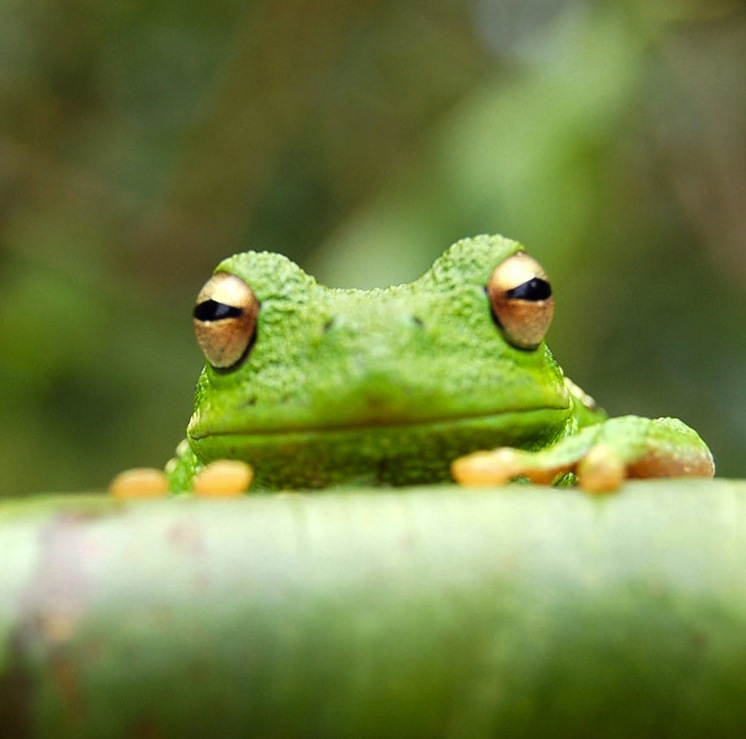
\includegraphics[width=0.5\textwidth]{frog.jpg}
%\caption{\label{fig:frog}This is a figure caption.}
%\end{figure}
%
%\begin{table}
%\centering
%\begin{tabular}{l|r}
%Item & Quantity \\\hline
%Widgets & 42 \\
%Gadgets & 13
%\end{tabular}
%\caption{\label{tab:widgets}An example table.}
%\end{table}
%
%\dots
%
%\begin{enumerate}
%\item Like this,
%\item and like this.
%\end{enumerate}
%\dots or bullet points \dots
%\begin{itemize}
%\item Like this,
%\item and like this.
%\end{itemize}

\end{document}
